\documentclass[11pt,a4paper]{article}

\usepackage[utf8x]{inputenc}   % omogoča uporabo slovenskih črk kodiranih v formatu UTF-8
\usepackage[slovene]{babel}    % naloži, med drugim, slovenske delilne vzorce

\usepackage{graphicx} % omogoča vključevanje slik


\title{Perspektiva}
\author{Aljoša Rakita\\
aljo.aljo.aljo@hotmail.com\\
\ \\
možni MENTOR:  prof. dr. Franc Solina  \\
Fakulteta za računalništvo in informatiko Univerze v Ljubljani
\date{\today}         
}


\begin{document}
\maketitle

Cilj te naloge je ugotoviti, kakšne so diplomske naloge na FRI, kakšne teme so možne in  katere teme pokrivajo posamezni mentorji.


\section{Motiv za diplomsko nalogo}

Zadnjih nekaj let je pri študentih arhitekture in likovnih smeri, ki so povezane z risanjem prostora po
načelih prostorskih ključev oziroma linearne perspektive, opaziti težave pri transferju realnega v
likovni prostor.

Podobno tematiko obravnavajo: 
\begin{itemize}

\item{Mobilna aplikacija za pomoč pri iskanju izdelkov v zaprtem prostoru} \cite{diploma1}.

\item{Mobilna aplikacija za razpoznavanje objektov iz več pogledov} \cite{diploma2}.

\item {Zasnova večkamernega sistema za priznavanje zadetka}  \cite{diploma3}.

\item {Podporna aplikacija za ornitologe}  \cite{diploma4}.


\end{itemize}

\section{Kaj je konkretni cilj diplomske naloge}

 Cilj je stvaritev vmesnika ki bi ob primerni uporabi v učnem
procesu, opozarjal na razlike med doživljanjem sveta prek vmesnikov in brez njih ter jim tako
omogočil lažje prehajanje iz realnega (skozi digitalni) v likovni prostor. 


\section{S kakšnimi orodji bomo prišli do uresničitve cilja}

Pri izdelavi diplomske naloge bomo večino dela naredili v razvojnem okolju Android studio, ki poenostavi razvoj mobilnih aplikacij.


\section{Kako bomo preizkusili rešitev ali ustreza zadanim ciljem}

Rešitev bomo predstavili tako, da bomo demonstrirali njeno delovanje na realnem primeru v realnem času.


\section{Vključevanje slik}

Prikaz delovanja aplikacije: slika \ref{fig:test}.


\begin{figure}[htb]
\begin{center}
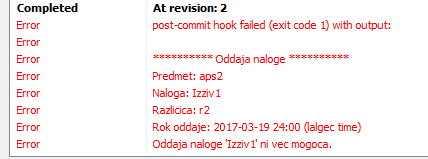
\includegraphics[width=0.8\columnwidth]{Capture}
\end{center}
\caption{Demonstracija delovanja}
\label{fig:test}
\end{figure}


\begin{thebibliography}{9}

\bibitem{diploma1}
Ariel David Jančar.
Mobilna aplikacija za pomoč pri iskanju izdelkov v zaprtem prostoru.
Diplomska naloga, Fakulteta za računalništvo in informatiko, Univerza v Ljubljani, 2018.

\bibitem{diploma2}
Matej Račič.
Mobilna aplikacija za razpoznavanje objektov iz več pogledov.
Diplomska naloga, Fakulteta za računalništvo in informatiko, Univerza v Ljubljani, 2017.

\bibitem{diploma3}
Jure Juvančič.
Zasnova večkamernega sistema za priznavanje zadetka.
Diplomska naloga, Fakulteta za računalništvo in informatiko, Univerza v Ljubljani, 2018.

\bibitem{diploma4}
Bojan Hameršak.
Podporna aplikacija za ornitologe.
Diplomska naloga, Fakulteta za računalništvo in informatiko, Univerza v Ljubljani, 2017.

\end{thebibliography}

\end{document}  




